\documentclass{report}

\usepackage{booktabs}
\usepackage[utf8]{inputenc}
\usepackage{graphicx}
\usepackage{pgfplots}
\usepackage[l3]{csvsimple}
\DeclareUnicodeCharacter{2212}{−}
\usepgfplotslibrary{groupplots,dateplot}
\usetikzlibrary{patterns,shapes.arrows}
\pgfplotsset{compat=newest}

\title{MATH 610 PA 3 Report}
\author{}
\date{}

\begin{document}
\maketitle
\chapter*{Problem 1}
% the error table should be organized first by final time, then by number of time steps, then by mesh size
% see https://docs.google.com/spreadsheets/d/11X0EiSMSQCzlYg5JUssQa9YV62GkJgdbgrtY774uoLg/edit?usp=sharing for an example
% uncomment and replace with csv file
\begin{figure}[h]
	\caption{Problem 1 error table}
	\csvautotabular{example.csv}
\end{figure}

\chapter*{Problem 2}
% plots should be organized first by final time, then by number of time steps, then by mesh size
% replace with plots and uncomment
\begin{figure}[h]
	\caption{Problem 2 $t = 1$ $n = 20$ $m = 10$}
	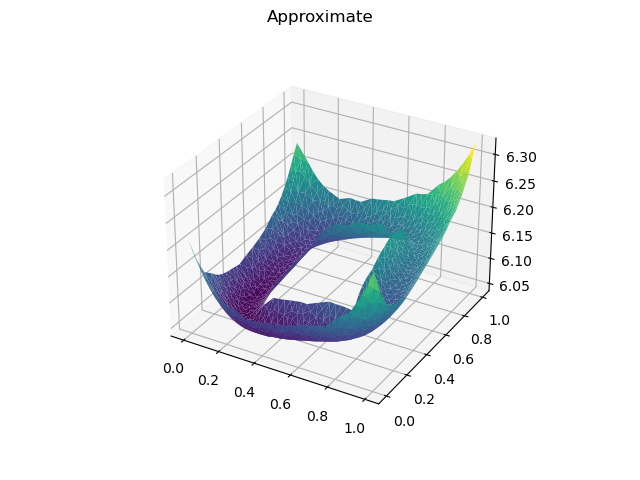
\includegraphics[width=\textwidth]{example.png}
\end{figure}
\begin{figure}[h]
	\caption{Problem 2 $t = 1$ $n = 20$ $m = 20$}
	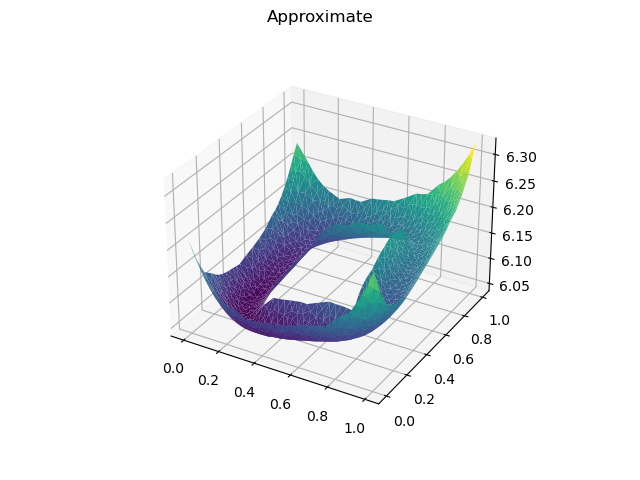
\includegraphics[width=\textwidth]{example.png}
\end{figure}
\begin{figure}[h]
	\caption{Problem 2 $t = 1$ $n = 20$ $m = 40$}
	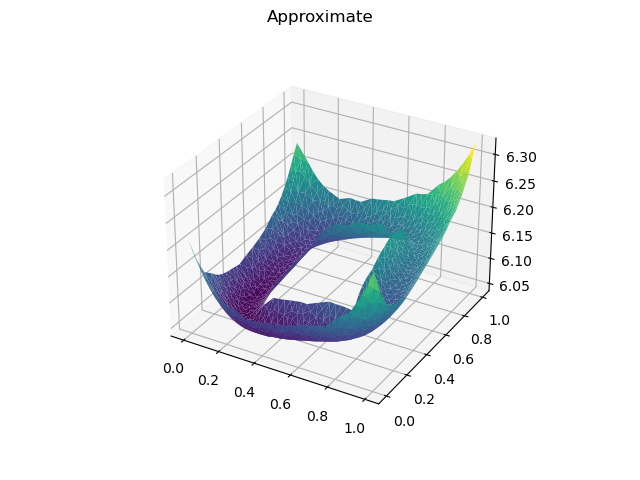
\includegraphics[width=\textwidth]{example.png}
\end{figure}
\begin{figure}[h]
	\caption{Problem 2 $t = 1$ $n = 40$ $m = 10$}
	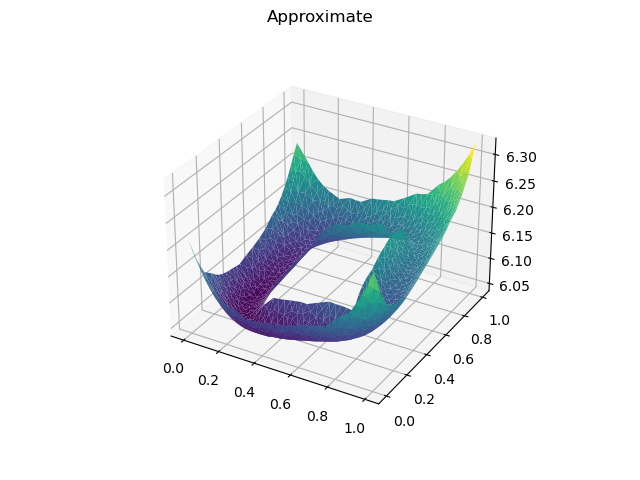
\includegraphics[width=\textwidth]{example.png}
\end{figure}
\begin{figure}[h]
	\caption{Problem 2 $t = 1$ $n = 40$ $m = 20$}
	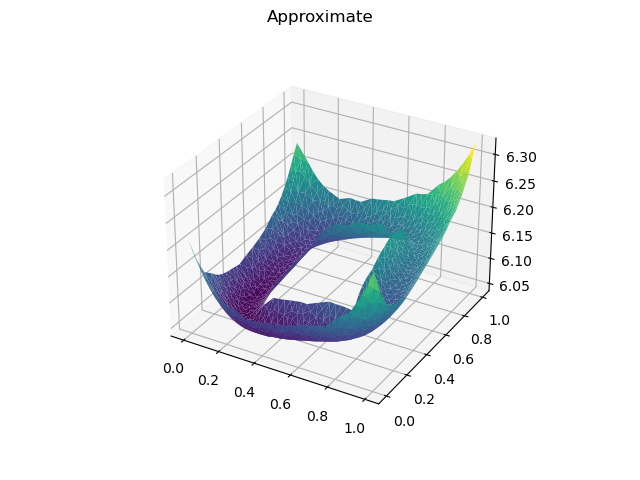
\includegraphics[width=\textwidth]{example.png}
\end{figure}
\begin{figure}[h]
	\caption{Problem 2 $t = 1$ $n = 40$ $m = 40$}
	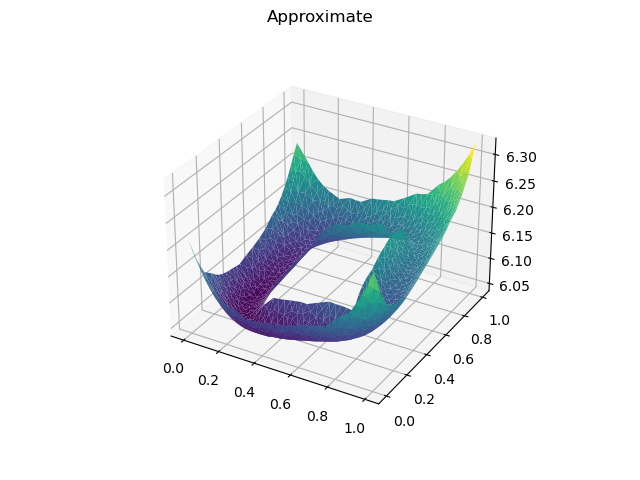
\includegraphics[width=\textwidth]{example.png}
\end{figure}
\begin{figure}[h]
	\caption{Problem 2 $t = 1$ $n = 80$ $m = 10$}
	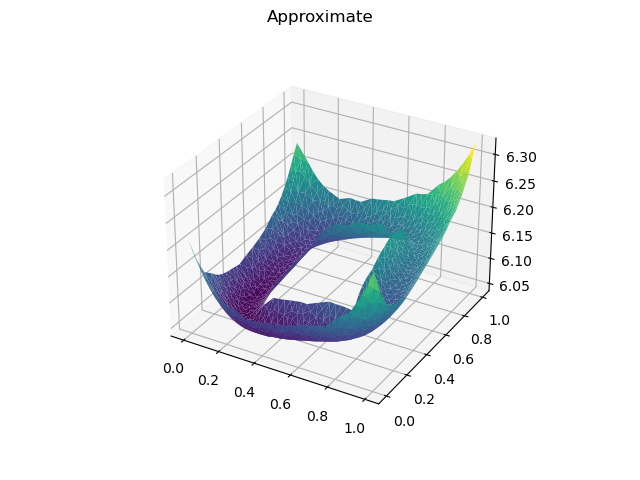
\includegraphics[width=\textwidth]{example.png}
\end{figure}
\begin{figure}[h]
	\caption{Problem 2 $t = 1$ $n = 80$ $m = 20$}
	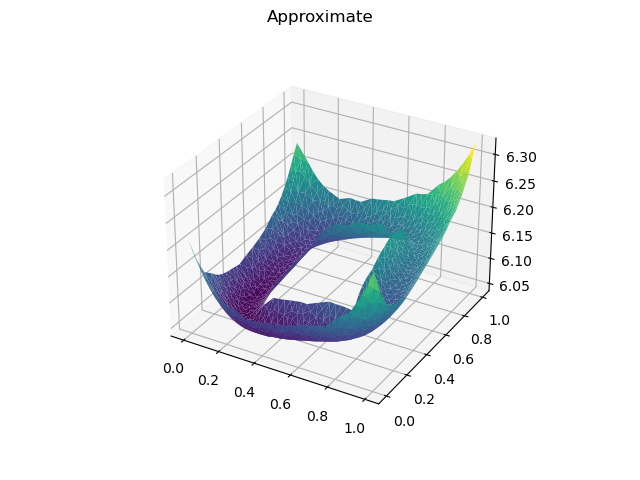
\includegraphics[width=\textwidth]{example.png}
\end{figure}
\begin{figure}[h]
	\caption{Problem 2 $t = 1$ $n = 80$ $m = 40$}
	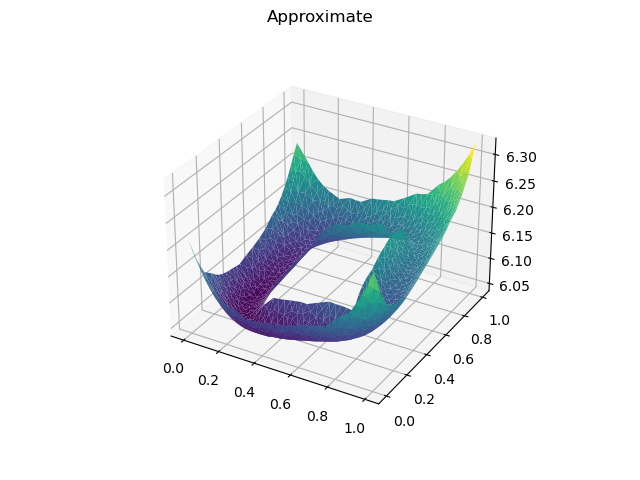
\includegraphics[width=\textwidth]{example.png}
\end{figure}
\begin{figure}[h]
	\caption{Problem 2 $t = 3$ $n = 20$ $m = 10$}
	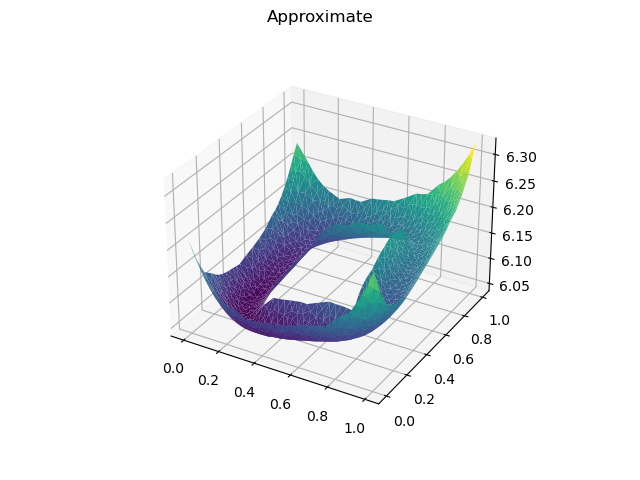
\includegraphics[width=\textwidth]{example.png}
\end{figure}
\begin{figure}[h]
	\caption{Problem 2 $t = 3$ $n = 20$ $m = 20$}
	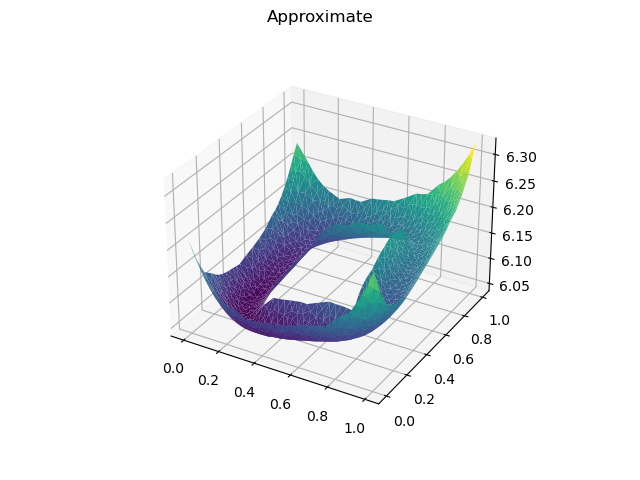
\includegraphics[width=\textwidth]{example.png}
\end{figure}
\begin{figure}[h]
	\caption{Problem 2 $t = 3$ $n = 20$ $m = 40$}
	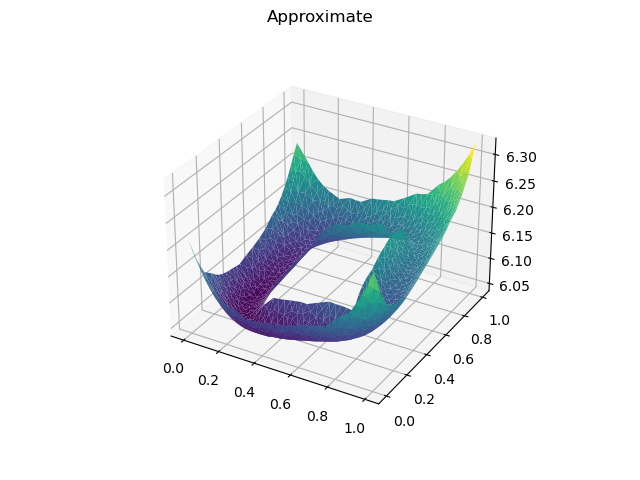
\includegraphics[width=\textwidth]{example.png}
\end{figure}
\begin{figure}[h]
	\caption{Problem 2 $t = 3$ $n = 40$ $m = 10$}
	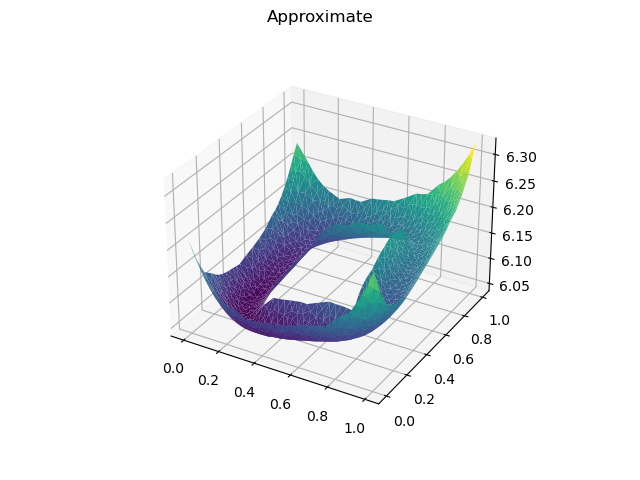
\includegraphics[width=\textwidth]{example.png}
\end{figure}
\begin{figure}[h]
	\caption{Problem 2 $t = 3$ $n = 40$ $m = 20$}
	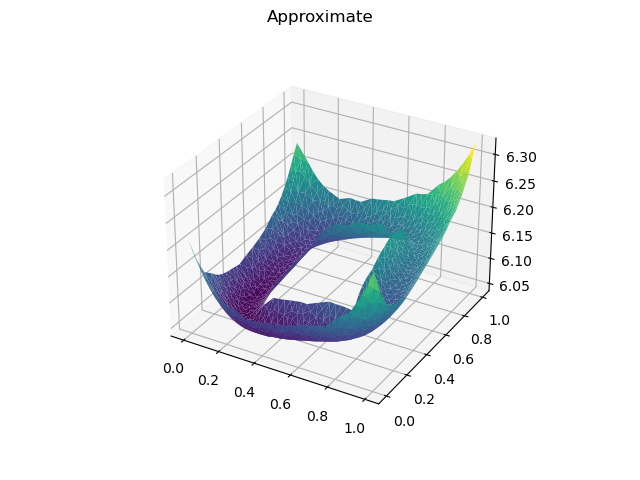
\includegraphics[width=\textwidth]{example.png}
\end{figure}
\begin{figure}[h]
	\caption{Problem 2 $t = 3$ $n = 40$ $m = 40$}
	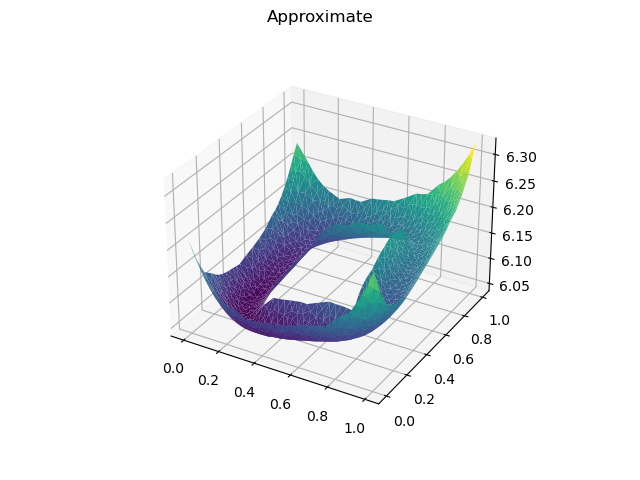
\includegraphics[width=\textwidth]{example.png}
\end{figure}
\begin{figure}[h]
	\caption{Problem 2 $t = 3$ $n = 80$ $m = 10$}
	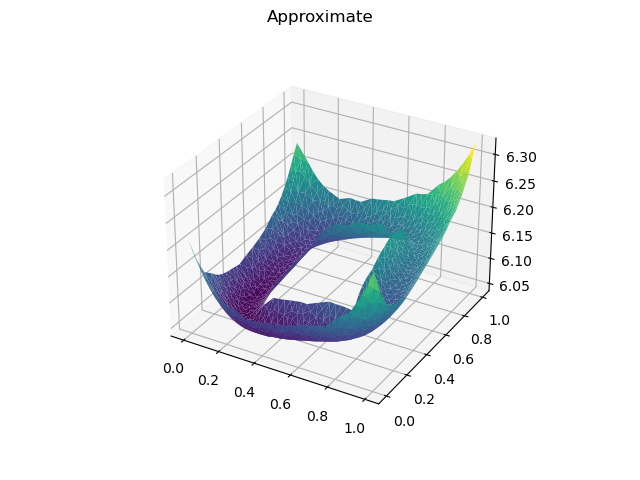
\includegraphics[width=\textwidth]{example.png}
\end{figure}
\begin{figure}[h]
	\caption{Problem 2 $t = 3$ $n = 80$ $m = 20$}
	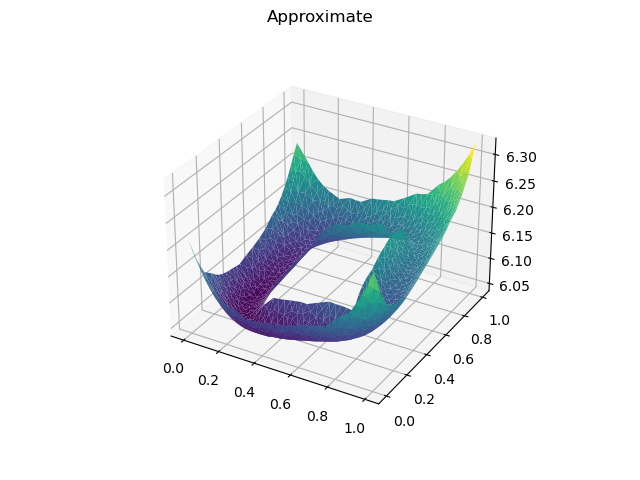
\includegraphics[width=\textwidth]{example.png}
\end{figure}
\begin{figure}[h]
	\caption{Problem 2 $t = 3$ $n = 80$ $m = 40$}
	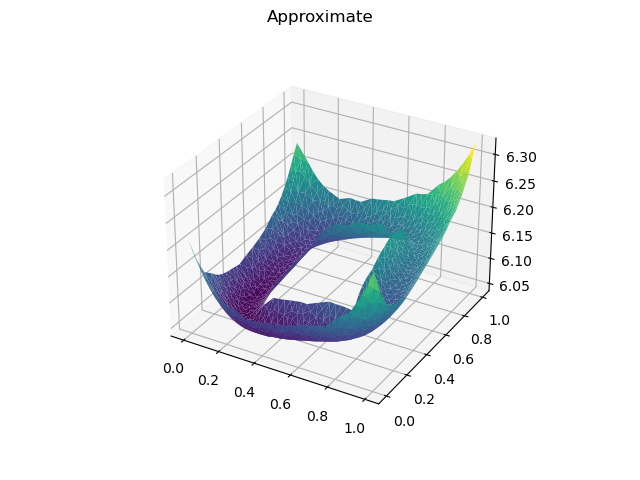
\includegraphics[width=\textwidth]{example.png}
\end{figure}


\chapter*{Problem 3}
% plots should be organized first by final time, then by number of time steps, then by mesh size
% replace with plots and uncomment
\begin{figure}[h]
	\caption{Problem 3 $t = 1$ $n = 20$ $m = 10$}
	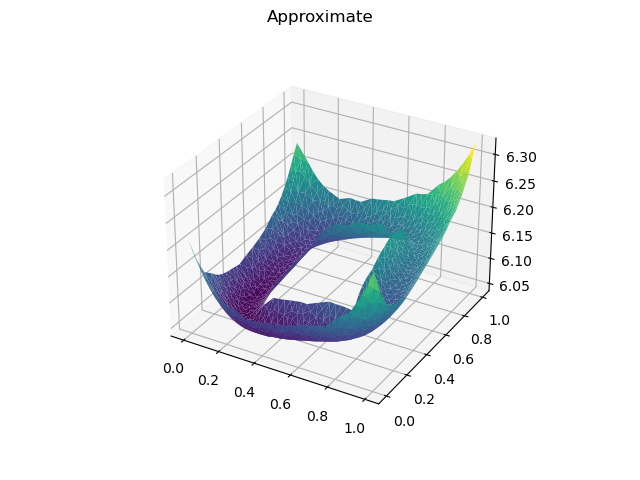
\includegraphics[width=\textwidth]{example.png}
\end{figure}
\begin{figure}[h]
	\caption{Problem 3 $t = 1$ $n = 20$ $m = 20$}
	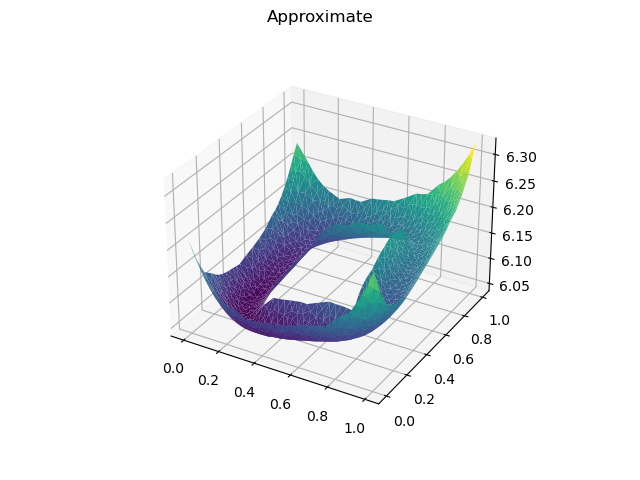
\includegraphics[width=\textwidth]{example.png}
\end{figure}
\begin{figure}[h]
	\caption{Problem 3 $t = 1$ $n = 20$ $m = 40$}
	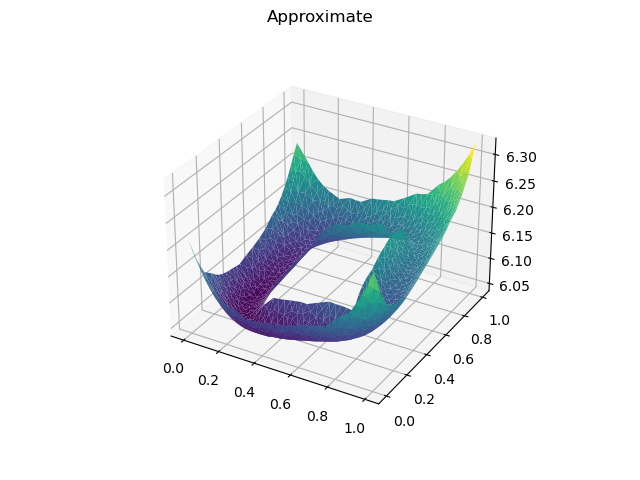
\includegraphics[width=\textwidth]{example.png}
\end{figure}
\begin{figure}[h]
	\caption{Problem 3 $t = 1$ $n = 40$ $m = 10$}
	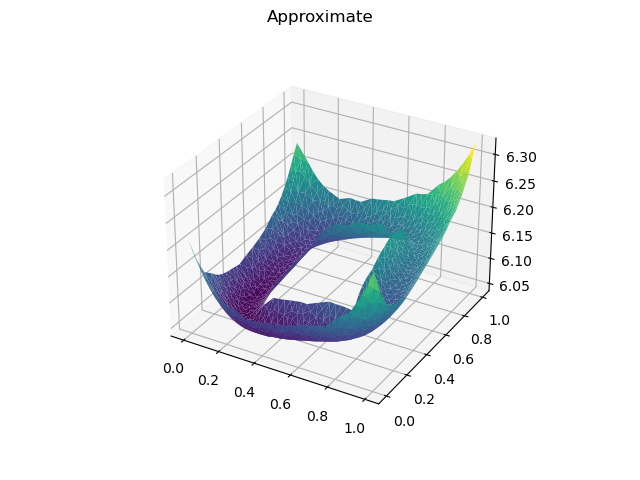
\includegraphics[width=\textwidth]{example.png}
\end{figure}
\begin{figure}[h]
	\caption{Problem 3 $t = 1$ $n = 40$ $m = 20$}
	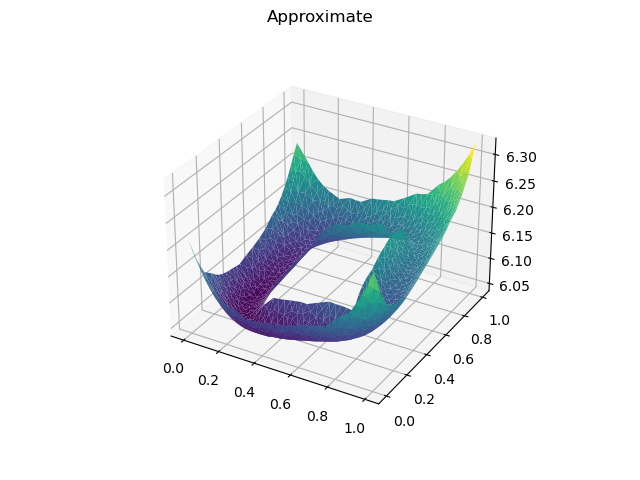
\includegraphics[width=\textwidth]{example.png}
\end{figure}
\begin{figure}[h]
	\caption{Problem 3 $t = 1$ $n = 40$ $m = 40$}
	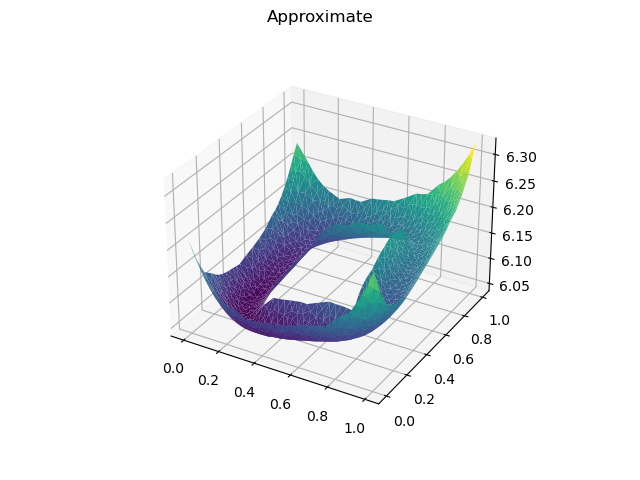
\includegraphics[width=\textwidth]{example.png}
\end{figure}
\begin{figure}[h]
	\caption{Problem 3 $t = 1$ $n = 80$ $m = 10$}
	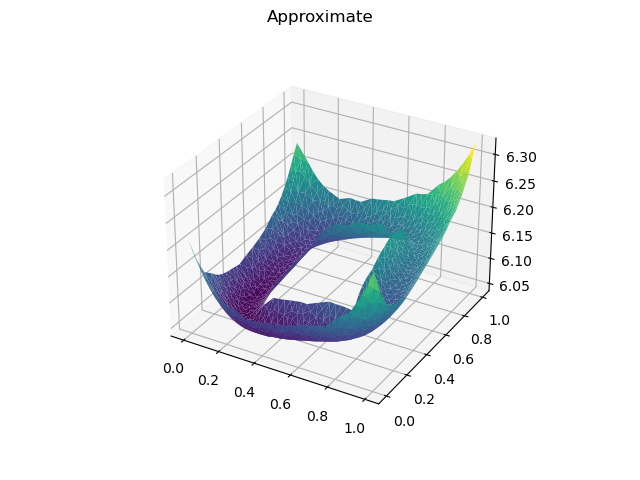
\includegraphics[width=\textwidth]{example.png}
\end{figure}
\begin{figure}[h]
	\caption{Problem 3 $t = 1$ $n = 80$ $m = 20$}
	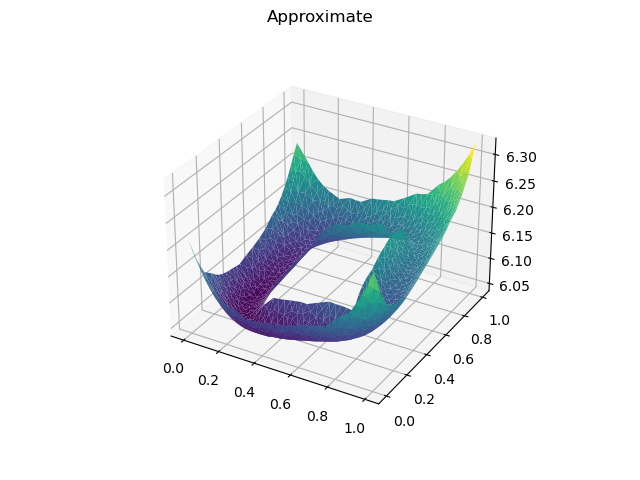
\includegraphics[width=\textwidth]{example.png}
\end{figure}
\begin{figure}[h]
	\caption{Problem 3 $t = 1$ $n = 80$ $m = 40$}
	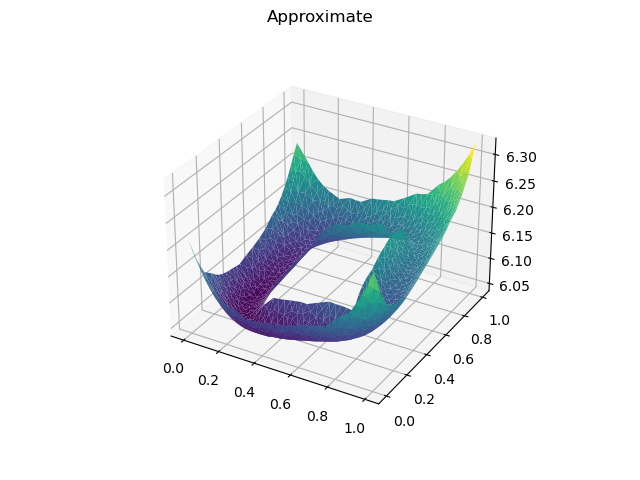
\includegraphics[width=\textwidth]{example.png}
\end{figure}
\begin{figure}[h]
	\caption{Problem 3 $t = 3$ $n = 20$ $m = 10$}
	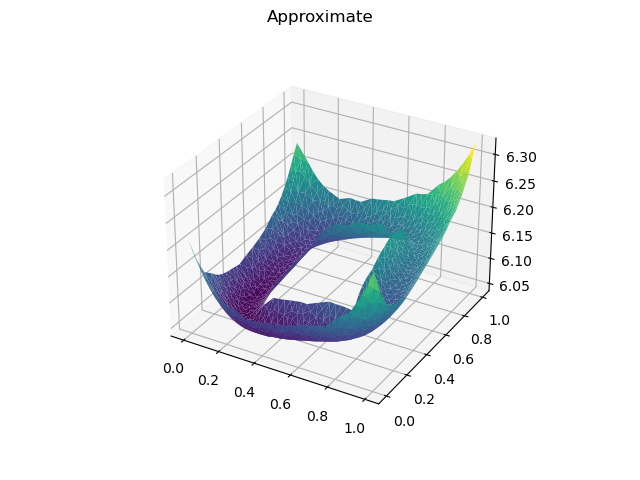
\includegraphics[width=\textwidth]{example.png}
\end{figure}
\begin{figure}[h]
	\caption{Problem 3 $t = 3$ $n = 20$ $m = 20$}
	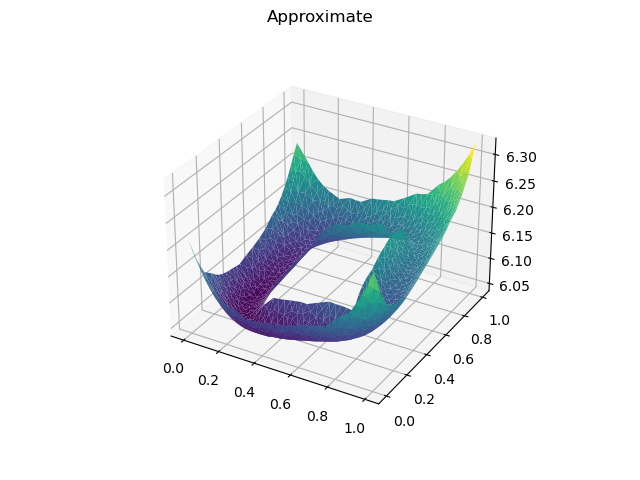
\includegraphics[width=\textwidth]{example.png}
\end{figure}
\begin{figure}[h]
	\caption{Problem 3 $t = 3$ $n = 20$ $m = 40$}
	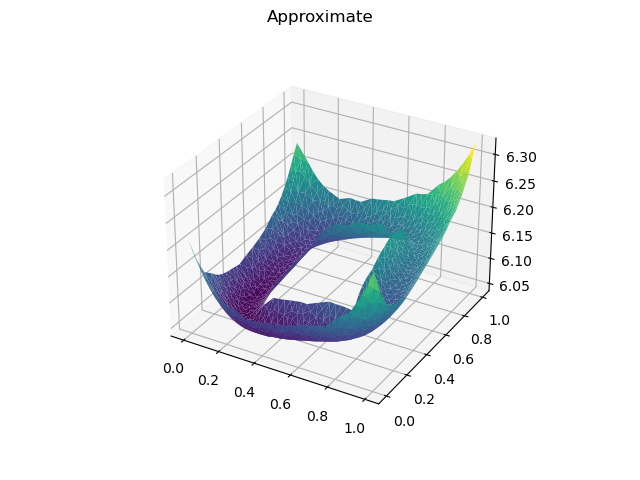
\includegraphics[width=\textwidth]{example.png}
\end{figure}
\begin{figure}[h]
	\caption{Problem 3 $t = 3$ $n = 40$ $m = 10$}
	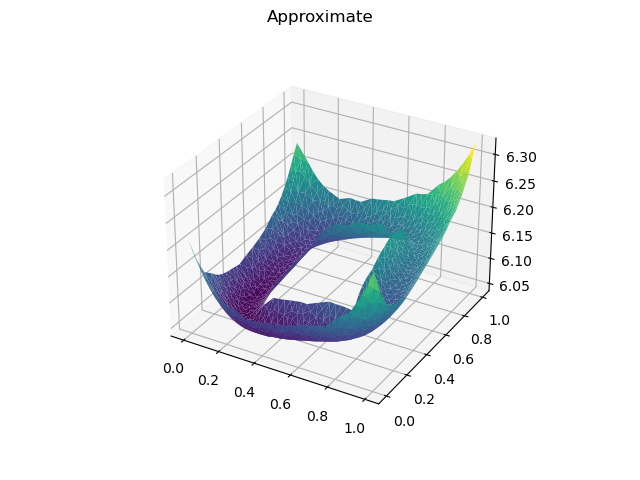
\includegraphics[width=\textwidth]{example.png}
\end{figure}
\begin{figure}[h]
	\caption{Problem 3 $t = 3$ $n = 40$ $m = 20$}
	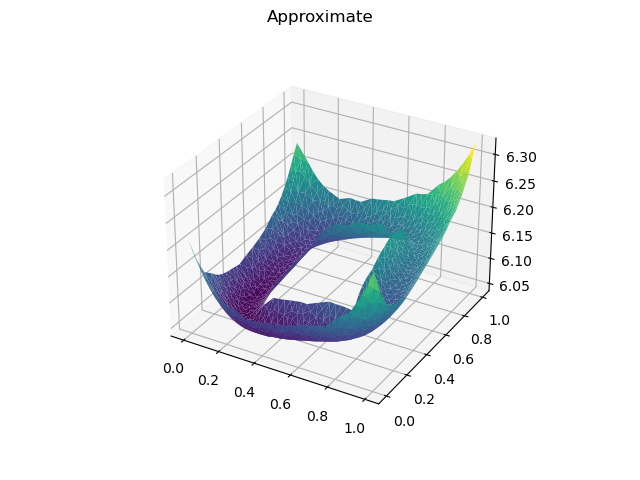
\includegraphics[width=\textwidth]{example.png}
\end{figure}
\begin{figure}[h]
	\caption{Problem 3 $t = 3$ $n = 40$ $m = 40$}
	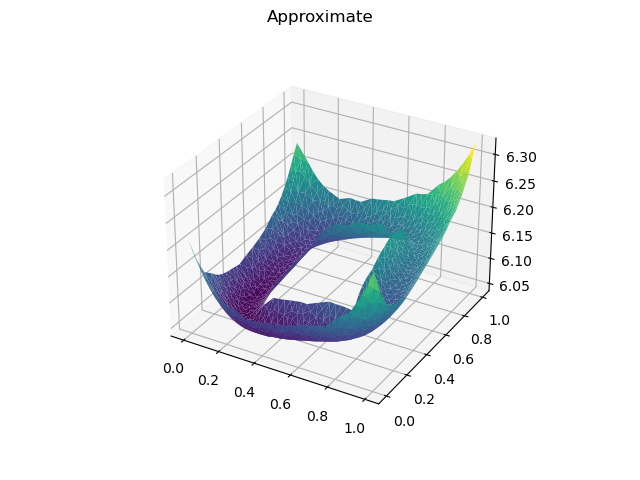
\includegraphics[width=\textwidth]{example.png}
\end{figure}
\begin{figure}[h]
	\caption{Problem 3 $t = 3$ $n = 80$ $m = 10$}
	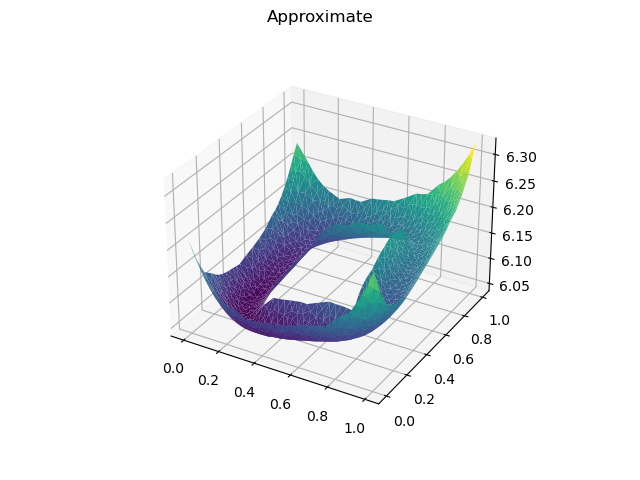
\includegraphics[width=\textwidth]{example.png}
\end{figure}
\begin{figure}[h]
	\caption{Problem 3 $t = 3$ $n = 80$ $m = 20$}
	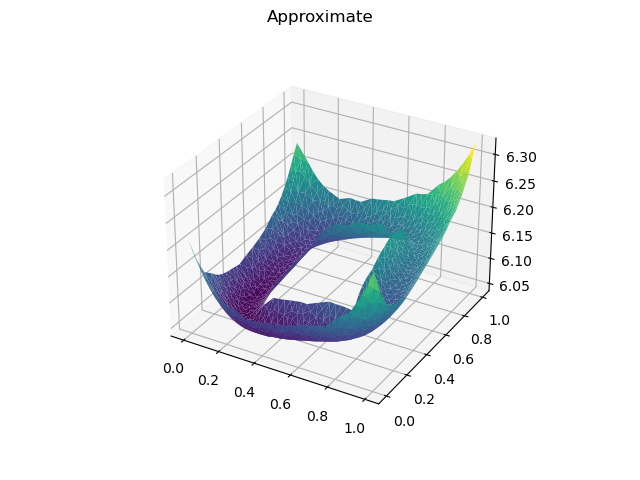
\includegraphics[width=\textwidth]{example.png}
\end{figure}
\begin{figure}[h]
	\caption{Problem 3 $t = 3$ $n = 80$ $m = 40$}
	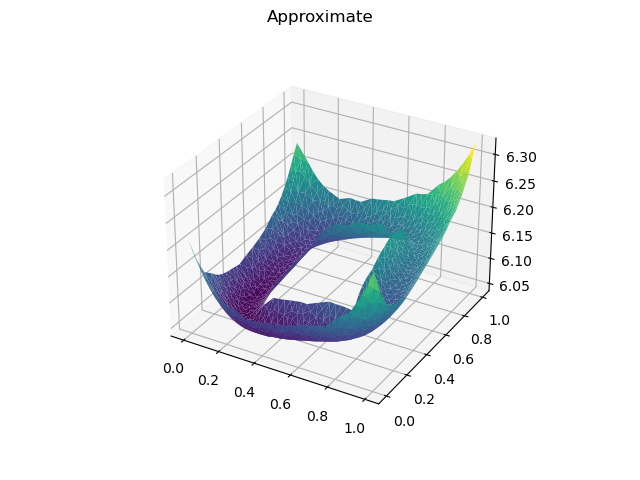
\includegraphics[width=\textwidth]{example.png}
\end{figure}
\end{document}
